\documentclass[parskip=full]{scrartcl}
\usepackage[utf8]{inputenc} % use utf8 file encoding for TeX sources
\usepackage[T1]{fontenc}    % avoid garbled Unicode text in pdf
\usepackage[german, english]{babel}  % german hyphenation, quotes, etc
\usepackage{graphicx}       % provides commands for including figures
\usepackage{rotating}
\graphicspath{ {images/} }
\usepackage{hyperref}       % detailed hyperlink/pdf configuration
\hypersetup{                % ‘texdoc hyperref‘ for options
pdftitle={PSE : LAMeetsML},%
bookmarks=true,%
}
\usepackage{csquotes}       % provides \enquote{} macro for "quotes"
\usepackage[nonumberlist, acronym]{glossaries} % provides glossary commands
\usepackage{enumitem}
\usepackage{lscape}
\usepackage{caption}
\usepackage{placeins}


\makenoidxglossaries
%
%%Glossary
%

\newglossaryentry{algorithm}
{
	name=algorithm,
	plural=algorithms,
	description={In mathematics and computer science, an algorithm is an unambiguous specification of how to solve a class of problems. Algorithms can perform calculation, data processing and automated reasoning tasks}
}

\newglossaryentry{classifier}
{
	name=classifier,
	plural= classifiers,
	description={The classifier is the last and main module in the program. It is able to determine the fastest \gls{preconditioner}/\gls{iterative solver} combination for a given sparse linear system. It uses the \gls{neural network} trained by the \gls{training module}}
}

\newglossaryentry{collector}
{
	name=collector,
	plural=collector,
	description={The collector is the first module in the program. Responsible for generating artificial matrices and collection preexisting matrices from the suite sparse matrix collection}
}

\newglossaryentry{command-line interface}
{
	name=command-line interface,
	plural=command-lines interface,
	description={A command-line interface is a means of interacting with a computer program where the user (or client) issues commands to the program in the form of successive lines of text (command lines). A program which handles the interface is called a command language interpreter}
}

\newglossaryentry{Ginkgo}
{
	name=Ginkgo,
	plural=Ginkgo,
	description={Ginkgo is a high-performance linear algebra library for manycore systems, with a focus on sparse solution of linear systems}
}

\newglossaryentry{GPU}
{
	name=GPU,
	plural=GPUs,
	description={A GPU is a graphic processing unit which has specialized electronic circuit designed to rapidly manipulate and alter memory to accelerate the creation of images in a frame buffer intended for output to a display device}
}

\newglossaryentry{grayscale sparsity pattern image}
{
	name=grayscale sparsity pattern image,
	plural=grayscale sparsity pattern images,
	description={Grayscale sparsity pattern image is an image, displaying the zero and nonzero areas of a matrix, by covering the zero areas white and all other areas by a shade of gray, depending on the value}
}

\newglossaryentry{iterative solver}
{
	name=iterative solver,
	plural=iterative solvers,
	description={In computational mathematics, an iterative solver does a mathematical procedure that uses an initial guess to generate a sequence of improving approximate solutions for a class of problems, in which the n-th approximation is derived from the previous ones}
}

\newglossaryentry{Keras}
{
	name=Keras,
	plural=Keras,
	description={Keras is an open source deep learning library written in Python}
}

\newglossaryentry{labeling module}
{
	name=labeling module,
	plural=labeling modules,
	description={The labeling module is the second module in the program. Responsible for executing a given set of matrices with all the \gls{preconditioner}/\gls{iterative solver}s combination specified. It will furthermore label each matrix with the fastest combination}
}

\newglossaryentry{Linux}
{
	name=Linux,
	plural=Linux,
	description={Linux is an open-source software operating systems}
}

\newglossaryentry{neural network}
{
	name=neural network,
	plural=neural networks,
	description={The neural network itself is not an \gls{algorithm}, but rather a framework for many different machine learning \glspl{algorithm} to work together and process complex data inputs. Such systems "learn" to perform tasks by considering examples, generally without being programmed with any task-specific rules}
}

\newglossaryentry{preconditioner}
{
	name=preconditioner,
	plural=preconditioners,
	description={In mathematics, preconditioning is the application of a transformation, that conditions a given problem into a form that is more suitable for numerical solving methods}
}

\newglossaryentry{Pytest}
{
	name=Pytest,
	plural=Pytests,
	description={Pytest is an alternative, more python fitting way of writing tests}
}

\newglossaryentry{Python}
{
	name=Python,
	plural=Python,
	description={Python is an interpreted high-level programming language for general-purpose programming}
}

\newglossaryentry{ResNet}
{
	name=resNet,
	plural=resNet,
	description={A deep residual network (deep ResNet) is a type of specialized neural network that helps to handle more sophisticated deep learning tasks and models}
}

\newglossaryentry{ssget}
{
	name=ssget,
	plural=ssget,
	description={Ssget is a command line tool for downloading matrices from the Suite Sparse Matrix Collection}
}

\newglossaryentry{Suite Sparse}
{
	name=Suite Sparse,
	plural=Suite Sparse,
	description={Suite Sparse is a suite of sparse matrix algorithms and Java interface to the Suite Sparse Matrix Collection}
}

\newglossaryentry{training module}
{
	name=training module,
	plural=training modules,
	description={The training module is the third module in the program. Responsible for training a deep neural network with the set of matrices and labels given by the \gls{labeling module}}
}

\newglossaryentry{Windows}
{
	name=Windows,
	plural=Windows,
	description={Microsoft Windows is a group of several graphical operating system families, all of which are developed, marketed, and sold by Microsoft}
}


\newglossaryentry{gaussian noise}
{
	name=gaussian noise,
	plural=gaussian noises,
	description={The gaussian noise is statistical noise having a probability density function equal to that of the normal distribution, which is also known as the Gaussian distribution. In other words, the values that the noise can take on are Gaussian-distributed}
}

\begin{document}

\begin{titlepage}
\centering
{\scshape\LARGE Karlsruher Institut für Technologie\par}
\vspace{1cm}
{\scshape\Large Functional Specification Document (FSD)\par}
\vspace{1.5cm}
{\huge\bfseries Numerical Linear Algebra meets Machine Learning \par}
\vspace {2cm}

{\Large\itshape Fabian Koffer\par}
{\Large\itshape Simon Hanselmann\par}
{\Large\itshape Yannick Funk\par}
{\Large\itshape Dennis Leon Gr\"{o}tzinger\par}
{\Large\itshape Anna Katharina Ricker\par}

\vfill
Supervisors\par
Hartwig Anzt
Makus G\"{o}tz

\vfill
{\large\today\par}
\end{titlepage}

\tableofcontents
\newpage


\section{Success Criteria}

Goal is the delivery of a consistent software stack that allows for employing 
\glspl{neural network} for the linear system. 
The ecosystem should allow to train a \gls{neural network} on selecting a suitable \gls{iterative solver} depending on the linear system characteristics.

\subsection{Mandatory Requirements}
\begin{itemize}

\item A software that supports the described work-flow design including the embedding of external components.

\item The software must be cross-platform compatible and support at least a \gls{Linux} and the \gls{Windows} operating system.

\item The software must be usable via a \gls{command-line interface} (CLI).

\item A data exchange format design that allows to store matrices and annotate them with 
additional meta-data, including labels.

\item An extensible design for multiple entities that are able to generate matrices in the proposed exchange format.

\item There need to be two actual realizations of these entities, which:

\begin{itemize}
    \item allow to generate artificial noise with uniform and \gls{gaussian noise} as well as
    
    \item can fetch test matrices from the \gls{Suite Sparse} matrix collection.
\end{itemize}

\item A dataset of at least 500 matrices in the envisioned data format and generated by the above two entities. There smallest share of matrices of a given entity must be no less than 30\% of the total number of contained matrices.

\item An extensible design that allows to solve the matrices using a configurable set of \gls{iterative solver} algorithms using a newly developed binding to the \gls{Ginkgo} linear algebra library.

\item A readily implemented and trained \gls{neural network} of the \gls{ResNet} architecture. It must be able to predict for a given matrix (in arbitrary format), which of the \gls{iterative solver} algorithms is the most suitable.

\item An entity that allows to store and load the trained \gls{neural network}.

\item The software must include entities for training and re-training a \gls{neural network} from scratch, respectively from a previously stored state.

\item The software must be able to show the predicted \gls{algorithm} and its associated suitability probability on the standard output.

\item Realization of a sustainable and quality-assured software development process. This includes a software design document, in-code documentation, unit testing and a continuous integration (CI).

\end{itemize}

\subsection{Optional Requirements}

\begin{itemize}
    
\item Scalability of the work-flow including matrix generation, training, prediction in that multiple processors may be used in parallel.

\item The software must be able to utilize \gls{GPU} accelerators for the training and prediction capabilities of the \gls{neural network}.

\item The system must support at least five \gls{iterative solver} \glspl{algorithm}.

\item A web interface to the software that is able to select a single, a set or all matrices of an uploadable file for prediction by the \gls{neural network}. The web interface may also be able to visualize the contained matrices, annotated labels as well as prediction results.

\end{itemize}

\subsection{Demarcation Criteria}
\begin{itemize}
\item No matrices other than sparse, square matrices will be supported

\item It should not be possible to program your own algorithms. Only access to existing algorithms is available.

\item Except for the matrices of \gls{Suite Sparse}, no other collections of matrices will be supported.

\end{itemize}
\section{Product use}
\subsection{Scope of application}
The software will be used for scientific work in the field of maths and computer science.
\subsection{Target groups}
Mathematicians and computer scientists who are working with sparse linear systems.
\subsection{Operating conditions}

\begin{itemize}
\item Use in the field of scientific work
\item Office environment
\end{itemize}

\section{Product environment}


\subsection{Software}
\begin{itemize}
\item The product will run on \gls{Windows} 10 and \gls{Linux} distributions 
\item The labeling of the matrices and training of the \gls{neural network} will be done with \gls{Linux}
\end{itemize}
\subsection{Hardware}

\begin{itemize}
\item The product will run on a workstation computer
\item The labeling of the matrices and training of the \gls{neural network} will be done on a server with multiple \glspl{GPU}
\end{itemize}

\subsection{Orgware}
A Documentation for the user will be generated.


\section{Functional requirements}
\subsection{Matrix Collecting}
	\begin{itemize}
	\item /F10/ Generation of sparse matrices by a given sparsity level and size
	\item /F15/ Generation of a given amount of matrices
	\item /F30/ Putting noise on the matrices
 	\item /F40/ Saving the generated matrices in a given directory
        \item /F50/ Choice to either only generate matrices or to generate some and fetch some from the \gls{Suite Sparse} matrix collection
	\item /F60/ Integration of the \gls{ssget} tool
	\end{itemize}
\subsection{Matrix Labeling}
	\begin{itemize}
	\item /F70/ Determination of the best solving \gls{algorithm} by time(fix \glspl{algorithm})
	\item /F71/ optional: Determination of the best solving \gls{algorithm} by time with custom \glspl{algorithm}
	\item /F75/ Labeling the matrix with the determined best algorithm
	\item /F90/ Creating a \gls{grayscale sparsity pattern image} of the labeled matrix
	\item /F100/ Saving the labeled matrix with its \gls{grayscale sparsity pattern image} in a given directory 
	\end{itemize}
	
	
\subsection{Deep \gls{neural network} Training and Testing}
	\begin{itemize}
	\item /F110/ Input of matrix files from a given directory
	\item /F120/ Randomization of the matrix files order
	\item /F125/ Separation of the matrix files into a training and testing dataset
	\item /F130/ Existence of a \gls{neural network} to train
	\item /F140/ Training of the \gls{neural network} by a given training dataset(/F125/)
	\item /F141/ Testing of the \gls{neural network} by a given testing dataset(/F125/)
	\item /F150/ Printing the accuracy(/loss) during the training and testing process of the \gls{neural network}
	\item /F151/ optional: creating of accuracy histograms
	\item /F160/ Loading a \gls{neural network} from a given directory
	\item /F161/ Saving the \gls{neural network} in its current state on a given directory
	\end{itemize}
 	
\subsection{Matrix Classification}
	\begin{itemize}
	\item /F170/ Input of a matrix to classify
	\item /F175/ Creating a \gls{grayscale sparsity pattern image} of the input matrix
	\item /F180/ Loading a trained \gls{neural network} from a given directory
	\item /F200/ Classification of the given \gls{grayscale sparsity pattern image} by the \gls{neural network}
	\item /F201/ Printing the classification output
	\end{itemize}

\section{Product data}
	\begin{itemize}
	\item artificial generated matrices
	\item collected matrices by \gls{ssget}
	\item 500-1000 labled matrices for training and test
	\item \gls{grayscale sparsity pattern image}
	\item \gls{neural network}

	\end{itemize}

\section{Nonfunctional requirements}
	\begin{itemize}
		\item /NF10/ All matrices are square
		\item /NF20/ All fixed \glspl{algorithm} are used within the labeling processes
		\item /NF30/ The \glspl{grayscale sparsity pattern image} all have the same size before training
		\item /NF40/ The \gls{neural network} ouputs a distinct prediction
		\item /NF50/ The \gls{neural network} is saved after every iteration
	\end{itemize}
	

\section{Global test cases}
\subsection{the following function sequences must be checked}
\subsubsection{Matrix Generation}
	\begin{itemize}
		\item /T10/ When generating a matrix, the returned matrix must have the right size and sparsity level
		\item /T15/ When generating a matrix, it must be square
		\item /T20/ When generating an amount of matrices, there must be an exact number of matrices by the given amount
		\item /T30/ When putting noise on a matrix, the returned matrix must have noise
		\item /T40/ After saving a matrix in the given directory, there must be the right file, with the right format
	\end{itemize}

\subsubsection{Matrix Labeling}
		\begin{itemize}
		\item /T50/ When labeling a Matrix, the label must be the \gls{algorithm} with the shortest time needed
		\item /T60/ When creating a \gls{grayscale sparsity pattern image} it must have the same size as
                       the matrix and must actually be grayscale
		\item /T70/ After saving the labeled matrix with its \gls{grayscale sparsity pattern image} in a given directory, there must be a file including the right matrix, the corresponding \glspl{grayscale sparsity pattern image} and the right label
		\end{itemize}
	\subsubsection{Deep \gls{neural network} Training and Testing}
		\begin{itemize}
		\item /T80/ When a matrix is loaded from a given directory, the right matrix must be loaded
		\item /T90/ When the matrix files are randomized they have to be in a different order after every randomization
		\item /T100/ After separating the dataset into a training and testing dataset, the training dataset must contain more matrices than the testing dataset
		\item /T110/ The \gls{neural network} has the right input dimensions for being trained by the matrices
		\item /T120/ The \gls{neural network} is only trained by the training dataset
		\item /T130/ The \gls{neural network} is only tested by the testing dataset
		\item /T140/ The printed loss(/accuracy) is the actual loss of the current training(/testing) iteration 
		\item /T150/ After saving the \gls{neural network} in its current state, there must be the right file in the right directory
		\end{itemize}
	\subsubsection{Matrix Classification}
		\begin{itemize}
		\item /T160/ After the input of a Matrix, the right file is loaded
		\item /T170/ After loading a \gls{neural network} from a given directory, the right \gls{neural network} has to be in the system
		\item /T180/ When printing the classification output, it has to be the prediction of the \gls{neural network}
		\end{itemize}
\newpage
\section{System models}
\subsection{Scenarios}
\subsubsection{Overview}
The product consists of four individual modules. The main module is the \gls{classifier} . Here the user may input a sparse matrix and receive the fastest \gls{preconditioner}/\gls{iterative solver} combination for solving the matrix. The user may furthermore interact with the other three modules; the \gls{collector}, the \gls{labeling module} and the \gls{neural network}.  Typical interaction with those modules will be described below.
\begin{center}
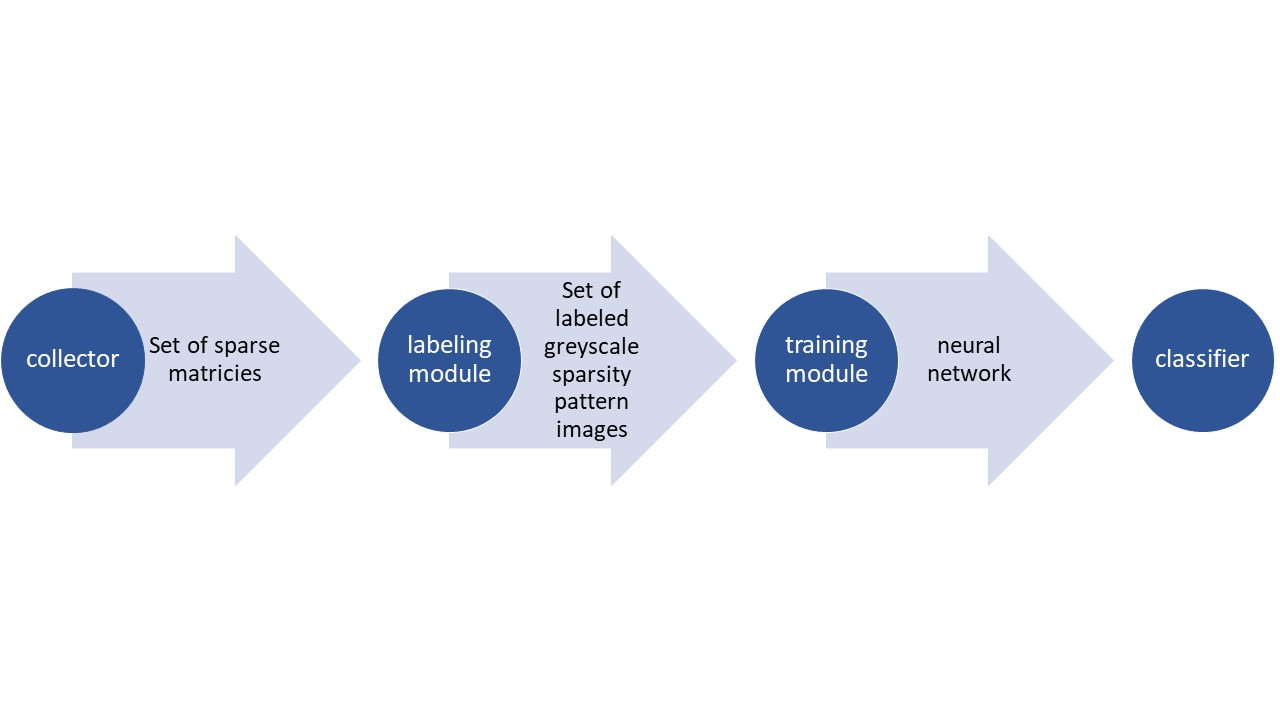
\includegraphics[width=\textwidth]{workflow}
\end{center}


\subsubsection{Use of the \gls{collector}}
The user wants a set of matrices for his own purpose. He likes our idea of combining the creation of matrices with fetching matrices from the \gls{Suite Sparse} matrix collection. He therefore opens the module \gls{collector}. He wants to generate 300 matrices of size 64x64 with a density of 0.2 and wants to use as many matrices as possible from the \gls{Suite Sparse} matrix collection. He wants to call his set of matrices collectedMatrices and enters the command \textit{collect -a 300 -n collectedMatrices -s 64 -d 0.2 -g}. When the process finished he gets notified. He navigates to the results file of the \gls{collector} in the file manager and proceeds with using the set of matricies for his own purposes.
\begin{center}
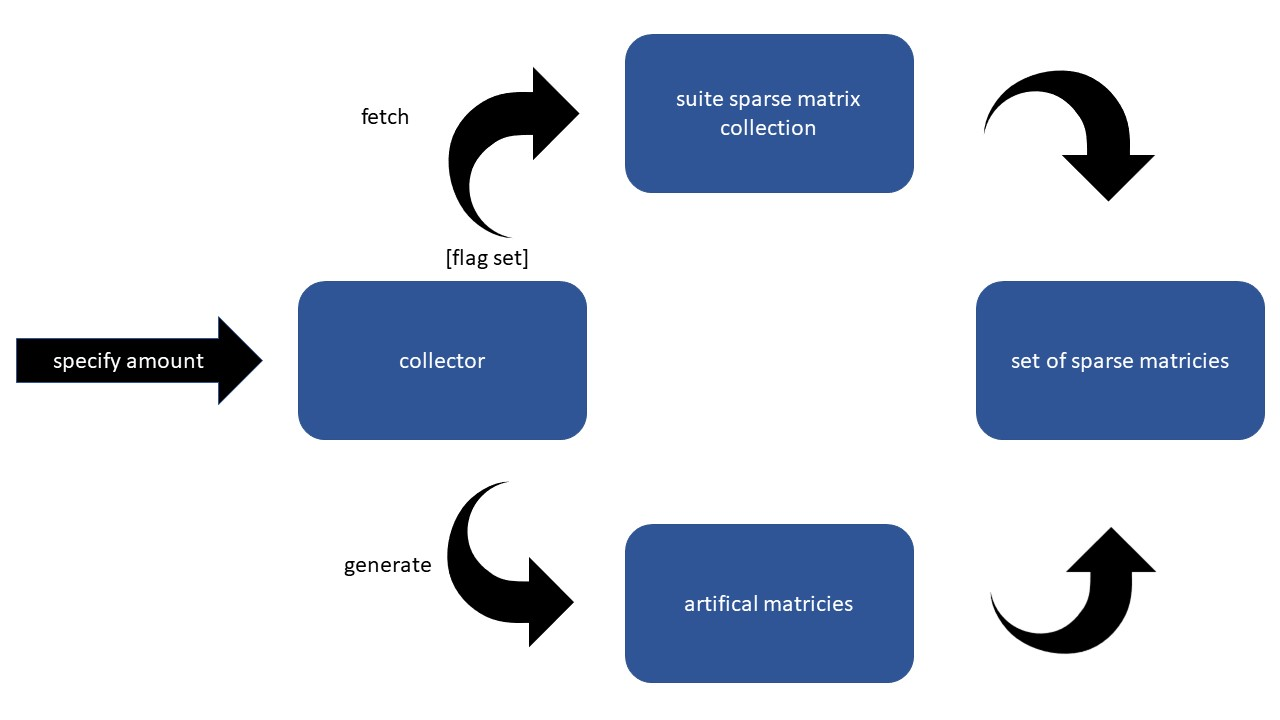
\includegraphics[width=\textwidth]{collector}
\end{center}

\subsubsection{Use of the \gls{labeling module}}
The user has a very specific problem which generates only a certain kind of sparse matrices. That is why he wants to adapt the \gls{neural network} for his specific task. He furthermore only wants to use the default \gls{preconditioner}/\gls{iterative solver} combinations. He first of all safes all of his matrices in one directory x of his choice. Then he opens the \gls{labeling module}. The command \textit{labeler label -p x -n labeledMatrices} will label all the matrices and generate their \gls{grayscale sparsity pattern image} in the directory. The set of \gls{grayscale sparsity pattern image} will be safed with the name labeledMatrices in the results file of the \gls{labeling module}. The user may proceed with using the \gls{neural network}.


\textbf{Optional:} The user is fine with the default matrices, but he wants to use other \gls{preconditioner}/\gls{iterative solver} combinations which are included in the \gls{Ginkgo} libary. He opens the \gls{labeling module}. With the command \textit{labeler list} he will see all the combinations that are currently used. With the command \textit{labeler add <\gls{preconditioner}/\gls{iterative solver}>} the new combinations of his choice will be added. With the command \textit{labeler remove <\gls{preconditioner}/\gls{iterative solver}>} the specified combination will be deleted. After the user made his choice he may proceed with using the \gls{neural network}.
\begin{center}
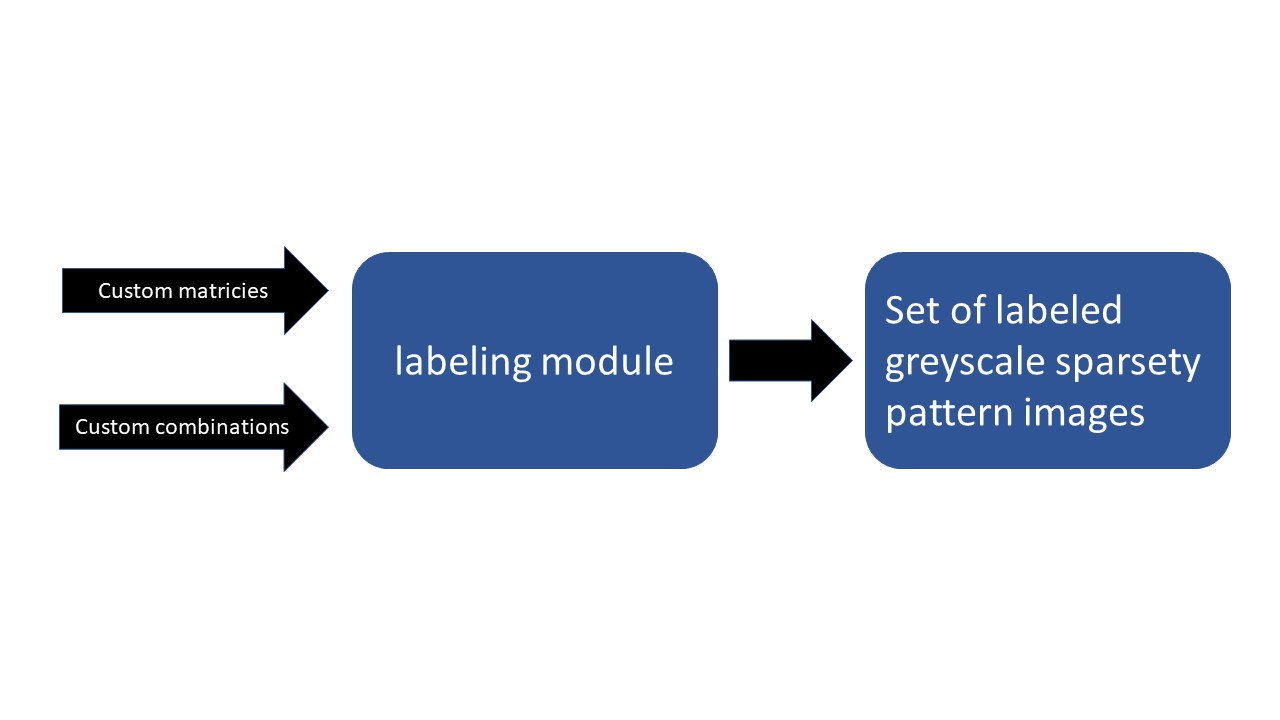
\includegraphics[width=\textwidth]{labelingModule}
\end{center}


\subsubsection{Use of the \gls{training module}}
\textbf{Optional:} The user has changed the set of matrices and/or the \gls{preconditioner}/\gls{iterative solver} combinations. He now wants to build the \gls{classifier}. He opens the \gls{training module}. With the command \textit{train -n myNeuralNetwork} the \gls{neural network} will be trained. The \gls{neural network} will be saved in the results folder with the name myNeuralNetwork.  The user may then proceed with using the \gls{classifier}.

\begin{center}
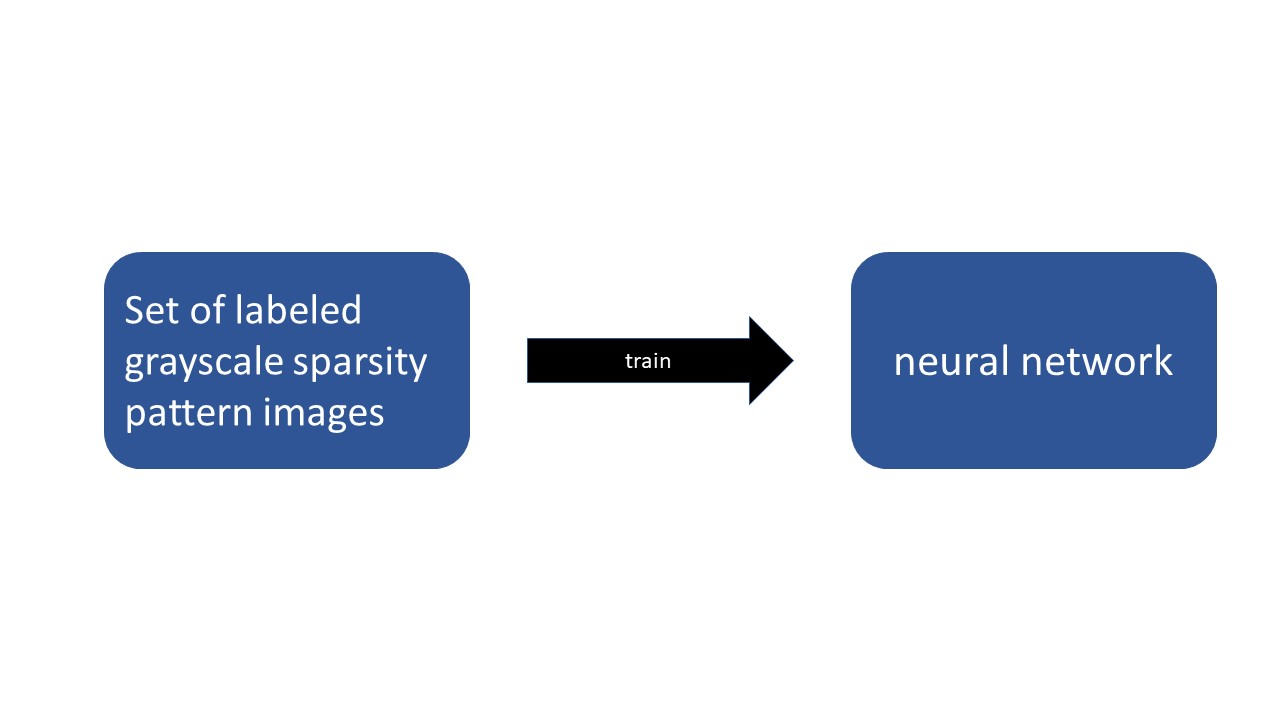
\includegraphics[width=\textwidth]{trainingModule}
\end{center}

\subsubsection{Use of the classifier}

The user wants to find the fastest \gls{preconditioner}/\gls{iterative solver} combination for a sparse linear system. If he did not change anything in the previous modules the default settings will be used. He will first save the sparse matrix in any desired filepath x. Afterwards the user starts the \gls{classifier}.
With the command \textit{classify  -p x - the \gls{neural network}} will classify the matrix and determine the fastest \gls{iterative solver}/\gls{preconditioner} combination for solving the matrix. This combination will be printed to the command line. (\textbf{Optional:} After determining the fastest combination the program will solve the matrix with this combination. The solved matrix will be safed in a directory the user specifies.)
\begin{center}
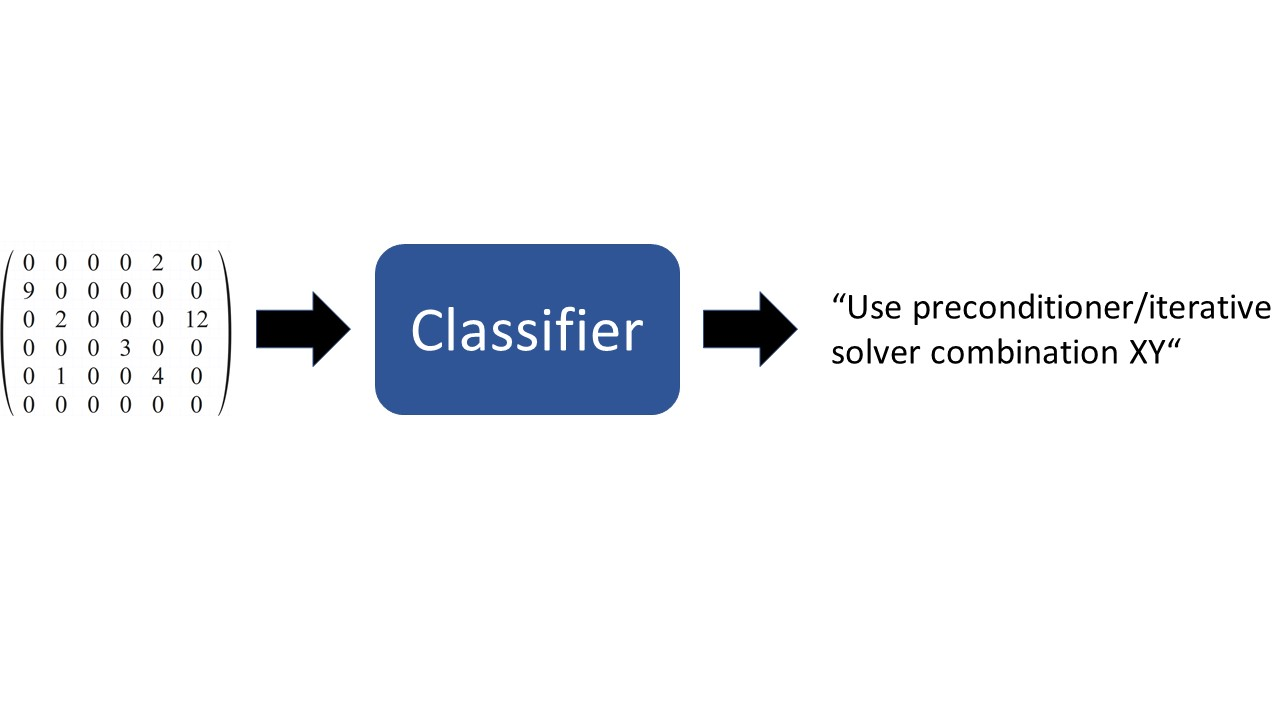
\includegraphics[width=\textwidth]{classifier}
\end{center}

\subsection{Use cases}
\subsubsection{Matrix \gls{collector}}
\includegraphics[width=1\textwidth]{useCase_collector_scaled}
\subsubsection{Matrix labeler}
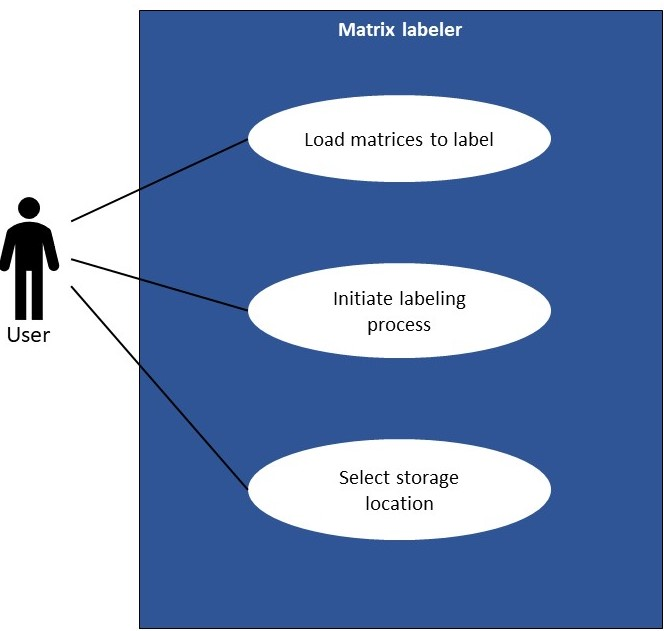
\includegraphics[width=1\textwidth]{useCase_Labeler_scaled}
\subsubsection{Neural network}
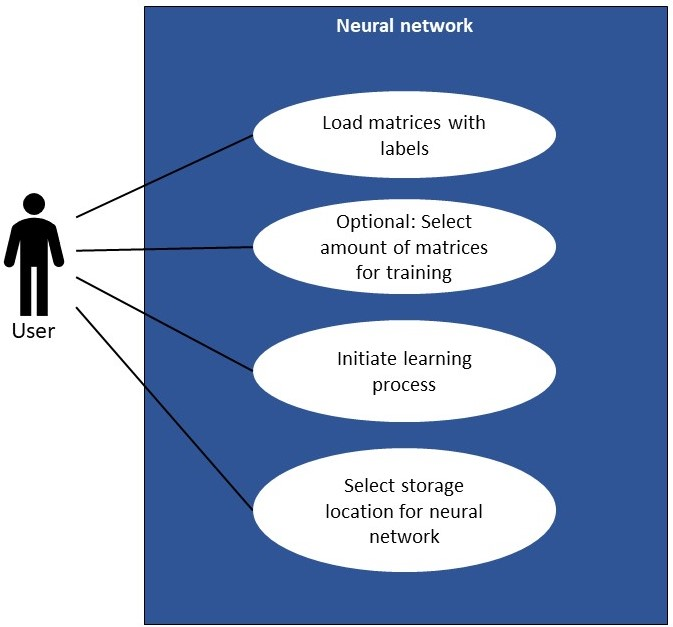
\includegraphics[width=1\textwidth]{useCase_NeuralNetwork_scaled}
\subsubsection{Classifier}
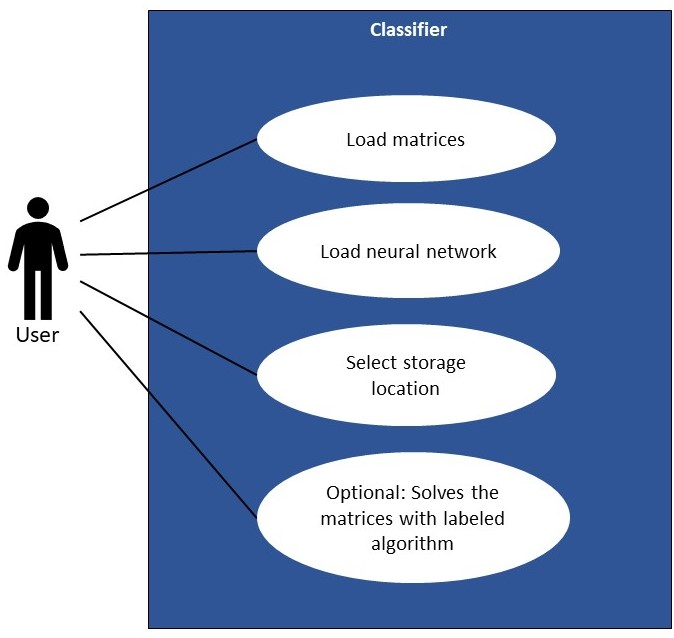
\includegraphics[width=1\textwidth]{useCase_Classifier_scaled}

\clearpage

\subsection{Command line options}
\begin{itemize}
\item/B10/\textbf{collect -a <amount> -n <name> -s <size> -d <density> -p <path> -g}:
\newline The user is able to create a specified amount of matrices that will be saved under a given name

\textbf{Arguments}
	\begin{itemize}
	\item[-]\textbf{-a <amount>} Absolute amount of matrices the user wants to generate
	\item[-]\textbf{-n <name>} Name under which the matrices will be saved
	\item[-]\textbf{-s <size>} (optional) Absolute size the generated square matrices should have. Default is 128
	\item[-]\textbf{-d <density>} (optional) Density level of the matrices. A float between 0 and 1 where 1 means no zero values. Default is 0.2
	\item[-]\textbf{-p <path>} (optional) Path where the created/downloaded matrices will be saved
	\item[-]\textbf{-g} (optional) (flag) If set it downloads as many matrices of that size as possible from the \gls{Suite Sparse} matrix collection
	\end{itemize}

\textbf{Print}
	\begin{itemize}
	\item[-]Progress notifying about the amount of matrices that are created and still need to be created
	\item[-]A message when process has finished with the path to the created matrices
	\item[-]Error, in case any required arguments are missing or invalid
	\item[-]Error, in case the specified name is already taken
	\item[-]Error, in case \textbf{-g} is set and user has no internet connection
	\item[-]Error, in case \textbf{-p <path>} is not a valid path
	\end{itemize}

\item/B20/\textbf{labeler label -p <path> -n <name> -s <saving path>}:
\newline The user is able to pass matrices that he wants to get labeled

\textbf{Arguments}
	\begin{itemize}
	\item[-]\textbf{label} (command) If set, enter labeling mode
	\item[-]\textbf{-p <path>} Absolute path to the matrices in the local storage the user wants to have labeled
	\item[-]\textbf{-n <name>} Name under which the labeled matrices will be saved
	\item[-]\textbf{-s <saving path>} (optional) Path where the labeled matrices will be saved
	\end{itemize}

\textbf{Print}
	\begin{itemize}
	\item[-]Progress notifying about the amount of matrices that are labeled and still need to be labeled
	\item[-]A message when process has finished with the path to the labeled matrices
	\item[-]Error, in case any required arguments are missing or invalid
	\item[-]Error, in case matrices have wrong format
	\item[-]Error, in case the specified name is already taken
	\item[-]Error, in case the remote fetching of the matrices did result in an error
	\item[-]Error, in case \textbf{-s <saving path>} is not a valid path
	\end{itemize}

\item/B30/\textbf{train -p <path> -n <name> -t <train> -s <saving path>}:
\newline The user is able to pass labeled matrices to a \gls{neural network}, that will learn from this matrices

\textbf{Arguments}
	\begin{itemize}
	\item[-]\textbf{-p <path>} Absolute path to the labeled matrices on the local storage
	\item[-]\textbf{-n <name>} Name under which the \glspl{neural network} will be saved after training has finished
	\item[-]\textbf{-t <train>} (optional) Float between 0 and 1. Amount of matrices used for training where 1 means all. Standard is 0.8
	\item[-]\textbf{-s <saving path>} (optional) Path where the \gls{neural network} state will be saved
	\end{itemize}

\textbf{Print}
	\begin{itemize}
	\item[-]Progress notifying about the loss of the current state based on test data
	\item[-]A message when process has finished with the path to the \gls{neural network} and the final loss
	\item[-]Error, in case any required arguments are missing or invalid
	\item[-]Error, in case matrices have wrong format or are not labeled
	\item[-]Error, in case the specified name is already taken
	\item[-]Error, in case \textbf{-s <saving path>} is not a valid path
	\end{itemize}

\item/B40/\textbf{classify -p <path> -n <network> -s}:
\newline The user is able to pass a matrix to the trained \gls{neural network}, which will find the best solving \gls{algorithm}.

\textbf{Arguments}
	\begin{itemize}
	\item[-]\textbf{-p <path>} Path to the matrix the user wants to classify
	\item[-]\textbf{-n <network>} (optional) Path to the trained \glspl{neural network}, if not set, uses the \gls{neural network} shipped with the program
	\item[-]\textbf{-s} (optional) (flag) If set matrix will also be solved after classification.
	\end{itemize}

\textbf{Print}
	\begin{itemize}
	\item[-]The \gls{preconditioner}/\gls{iterative solver} combination which will solve the given matrix the fastest
	\item[-](optional) The solved matrix
	\item[-]Error, in case any required arguments are missing or invalid
	\item[-]Error, in case the matrix has a wrong format
	\item[-]Error, in case the \gls{neural network} or matrix path is wrong
	\end{itemize}

\item(optional)/B50/\textbf{labeler list}:
\newline The user is able to retrieve a list of the available and used algorithms for the labeling module

\textbf{Arguments}
	\begin{itemize}
	\item[-]\textbf{list} (command) If set, enter list mode
	\end{itemize}

\textbf{Print}
	\begin{itemize}
	\item[-]A list of all \glspl{algorithm} the \gls{labeling module} currently uses and is able to use
	\item[-]Error, in case the user passed more arguments
	\end{itemize}

\item(optional)/B60/\textbf{label add <algorithm>}:
\newline The user is able to add an \gls{algorithm} that will be used for labeling matrices.

\textbf{Arguments}
	\begin{itemize}
	\item[-]\textbf{add} (command) If set, enter adding mode
	\item[-]\textbf{<algorithm>} A list of all \glspl{algorithm} the user wants to add, separated by blanks
	\end{itemize}
\textbf{Print}
	\begin{itemize}
	\item[-]A message if the adding worked
	\item[-]Error, in case the entered \gls{algorithm}/\glspl{algorithm} is not supported 
	\item[-]Error, in case other arguments were passed
	\end{itemize}

\item(optional)/B70/\textbf{label remove <algorithm>}:
\newline The user is able to remove an \gls{algorithm} from the list of used algorithms.

\textbf{Arguments}
	\begin{itemize}
	\item[-]\textbf{remove}(Command) If set, enter removing mode
	\item[-]\textbf{<algorithm>}A list of \glspl{algorithm} the user wants to remove from the used algorithms
	\end{itemize}
\textbf{Print}
	\begin{itemize}
	\item[-]A message if the removing worked
	\item[-]Error, in case the entered \gls{algorithm}/\glspl{algorithm} is not found. 
	\item[-]Error, in case other arguments were passed
	\end{itemize}

\end{itemize}
\clearpage

\section{Feasibility Study}
\subsection{Technical Feasibility}
There exist programs that try to solve the same problem, but with different approaches. 
Most of them scan the matrices for special metrics and based on that decide which solver will be the fastest. 
So there are metrics the \gls{neural network} might find, to predict the optimal solver for a given matrix. 
Other than that, most of the things needed can already be found in plugins like Keras for the \gls{neural network} and \gls{ssget} for downloading matrices from the \gls{Suite Sparse}. 
So there definitely is a way to accomplish this task and the only question is how accurate the \gls{classifier} will be.

\subsection{Alternatives}
As mentioned before, there are programs that try to solve the same problem and some of them are also quite accurate at it.
But for the moment nobody can tell if our approach might be more accurate.

\subsection{Personal Feasibility}
The team consists of five trained computer scientists with some of them already having experience regarding machine learning techniques.
There are also two experts that can be contacted when the team needs some help with more difficult questions.

\subsection{Legal Feasibility}
Since the team uses the 2-Clause BSD License for their written software, there is legal feasibility because the team holds the sole
copyright to their project but is not responsible for any consequential damage, caused by the use of their software.
\clearpage

\section{Glossary}
%\glspl{collector}, labeling modle, neural network, classifier, default settings  \glspl{Dateiformat}

% % Automatisch generiertes Glossar (Latex zwei mal ausführen um Glossar anzuzeigen)
%
%\glsaddall % das sorgt dafür, dass alles Glossareinträge gedruckt werden, nicht nur die verwendeten. Das sollte nicht nötig sein!
\printnoidxglossaries

\end{document}
